\section{Physical Layer-based Security}


\subsection{Channel-based Key Establishment}

\paragraph{Unique channels}
In a complex, multi-path rich environment channel exhibit time-varying, stochastic and reciprocal fading.
For receivers separated by $> \lambda / 2$ their channels are \underline{not} correlated.

Thus the channels between sender $S$ and receiver $R$ are ``random'' and cannot be known/predicted by the attacker.
In particular, the attacker cannot remotely measure multipath fading components of the signal strength.

\paragraph{Key Agreement through Channel Properties}
We can leverage different properties of the channel, e.g. RSSI\footnote{Received Signal Strength Indication}, CIR\footnote{Carrier-to-interference ratio} or signal phase.

The generic steps are the following:
\begin{enumerate}
	\item Signal Acquisition and Quantisation
	\item Reconciliation (error correction, privacy amplification)
	\item Key confirmation
\end{enumerate}

\begin{figure}[h]
	\centering
	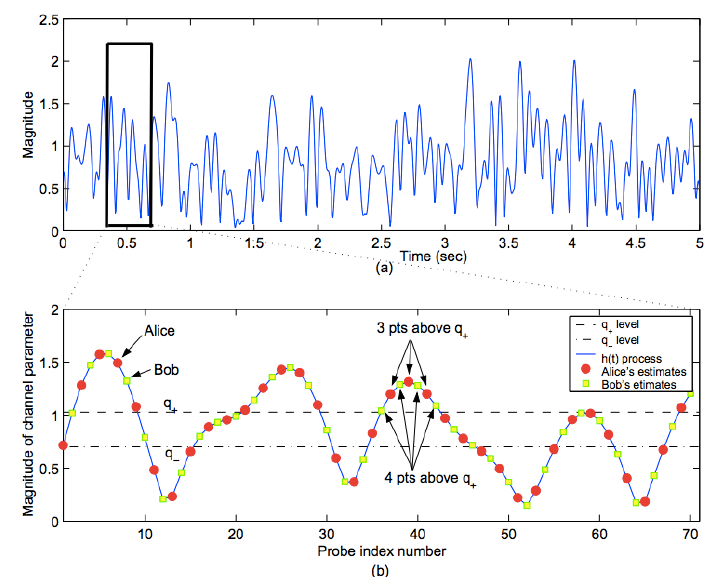
\includegraphics[scale=0.5]{images/7-channel-property.png}
	\caption{Measuring Channel Property Magnitudes over Time}
	\label{fig:channel-property}
\end{figure}

\paragraph{Analysis}
There are several disadvantages to this scheme:
\begin{itemize}
	\item No authentication: we establish a secret key, but with whom?
	\item No guarantees on the environment:
	Multi-path rich? Cannot be pre-measured? Receivers (and attacker!) at least $> \lambda / 2$ from each other?
	\item Questionable benefit over classic public-private-key schemes (no information-theoretic security)
	\item Active attacker not considered: can influence and discover the key
\end{itemize}

\paragraph{Ensuring Secrecy with MIMO}
\underline{Goal}: strengthen the security of the previous scheme.
\\
\underline{Idea}: use multiple antennas on both ends, to
(a) steer the signal towards the receiver and away from the attacker and
(b) use jamming to interfere with the attacker (but not the receiver).

Note that we can model each channel (or the signal on that channel) as a complex number (amplitude as the real part, phase as the imaginary part).

\paragraph{Zero Forcing}
Assumption: $S$ knows the channels to the intended receiver $R_1$ and to the attackers $R_2, R_3$, which are given as channel matrices $H_r$.
The sender applies a transmission filter $F$ that is constructed such that $R_r = H F D = H S$ contains useful data for $R_1$ but not for the attackers.

\paragraph{Orthogonal Blinding}
Same as zero forcing, but we only assume that the channel to the intended receiver $R_1$ is known (but not the channels to the attacker).
Construct the filter $F$ such that for everybody but $R_1$ the result $R_r$ contains a jamming signal (i.e. noise).

\begin{figure}
	\centering
	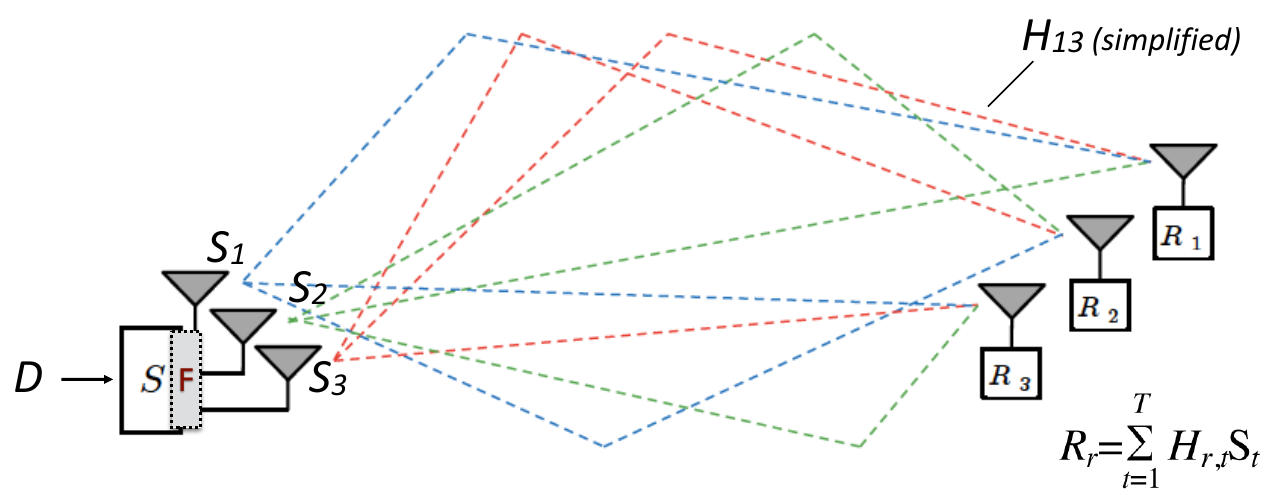
\includegraphics[scale=0.3]{images/7-mimo.png}
	\caption{MIMO channel}
	\label{fig:mimo}
\end{figure}

\paragraph{Analysis}
\begin{itemize}
	\item[$\oplus$] Stronger guarantees than SISO (beam forming focusses energy on receiver, jamming interferes with attacker)
	\item[$\ominus$] Still no authentication
	\item[$\ominus$] Still no guarantees on environment
	\item[$\ominus$] Still questionable benefit over classic public-private-key
	 schemes
	\item[$\ominus$] Passive attack: known plaintext attack (attacker can train filter)
	\item[$\ominus$] Active attack: abuse lack of authentication
\end{itemize}


\subsection{Friendly Jamming for Confidentiality and Access Control}

\paragraph{Friendly Jamming}
Transmit noise that the receiver can subtract (assuming a shared secret -- possibly established with one of the earlier methods).%
\footnote{Note the difference to orthogonal blinding, which does not add noise to all channels but only to the null space of the receiver's channel.}
The attacker on the other hand cannot distinguish signal and noise.

Example: IMD Shield for implanted medical devices.

\paragraph{Analysis} (as claimed by the IMD Shield paper). \\
Let $DJ$ be the distance between the data and jamming antenna (of the sender).
If $DJ > \lambda/2$ then an attacker with two antennas can separate the two signals (multiple channels).
Furthermore, if $DJ >> \lambda/2$ then the attacker can use directional antennas for signal separation.
\\
Thus the only ``safe'' case is $DJ < \lambda/2$ (i.e. when channels from D to A and from J to A are highly correlated).

However, this does NOT hold:
a MIMO attacker can retrieve the data even when $DJ < \lambda/2$, see the following:

\paragraph{Attack in Line of Sight LOS Model} 
The attacker places two antennas $A, B$ (see \autoref{fig:friendly-jamming-attack}).
The ideal placement is such that they receive both the jamming signal simultaneously (e.g. equidistant to the jammer) and the data signals with a phase shift of $\lambda/2$.
However, even with imperfect placement some data can still be recovered (with some attenuation).

When we also consider multipath effects (additional changes in amplitude and phase offsets) the attack becomes much harder.

\begin{figure}
	\centering
	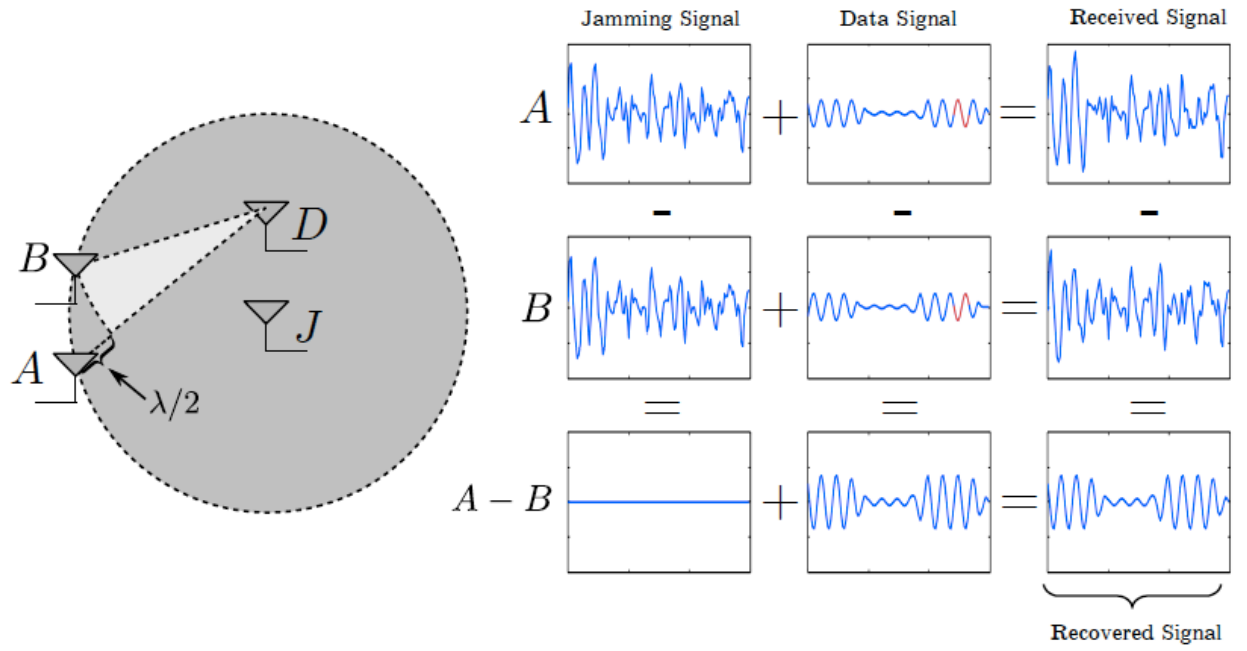
\includegraphics[scale=0.4]{images/7-friendly-jamming-attack.png}
	\caption{Friendly Jamming Attack Through Antenna Placement}
	\label{fig:friendly-jamming-attack}
\end{figure}

\paragraph{Conclusion}
Jamming works well for access control (in the sense that $J$ prevents malicious signals being send to $D$).
It does NOT work for confidentiality since a MIMO attacker can retrieve data even when $DJ < \lambda/2$.

In other words, the IMD Shield protects against malicious commands being sent to the implant, but not against an attacker listening to outgoing signals.

\paragraph{Signal Annihilation}
An attacker can deliberately introduce destructive interference to attenuate a legitimate signal.

Note that this is different to jamming!
Here, we are fooling the receiver to believe that there is \underline{no} signal on the channel.

\paragraph{Summary}
\begin{itemize}
	\item Using the physical layer for access control seems realistic.
	\item Using it for confidentiality however is questionable!
	Weak guarantees, use only as complementary measures.
\end{itemize}


\subsection{Broadcast Authentication: Presence Awareness}

\paragraph{Scenario}
One broadcasting station, many receivers.
No pre-shared keys, no credentials (certificates, public keys, etc).
Receivers know that they are within the power range of the legitimate sender 
(reasonable in airports, universities, etc).
Receivers know which channel (frequency) the sender is broadcasting.
The sender is always on and transmitting.

\underline{Goal}: distinguish between broadcast messages of legitimate and malicious station.
In other words, a physical layer-based broadcast authentication scheme based on presence awareness.
See also \autoref{sec:broadcast-auth}.

\paragraph{Integrity Codes Protocol} \mbox{}\\
\underline{Sender:}
Spread message $m$ from $k$ to $2k$ bits using Manchester encoding (1 $\rightarrow$ 10, 0 $\rightarrow$ 01).
Transmit result using on-off keying.
\\
\underline{Receiver:}
Set power thresholds above which to interpret a signal as 1. Then decode.
\\
\underline{Integrity Verification:}
Check if hamming weight%
\footnote{Recall that the hamming weight is the number of bits unequal to 0.}
$H(m)=|m|/2$. If yes, the message was not modified.

\begin{figure}
	\centering
	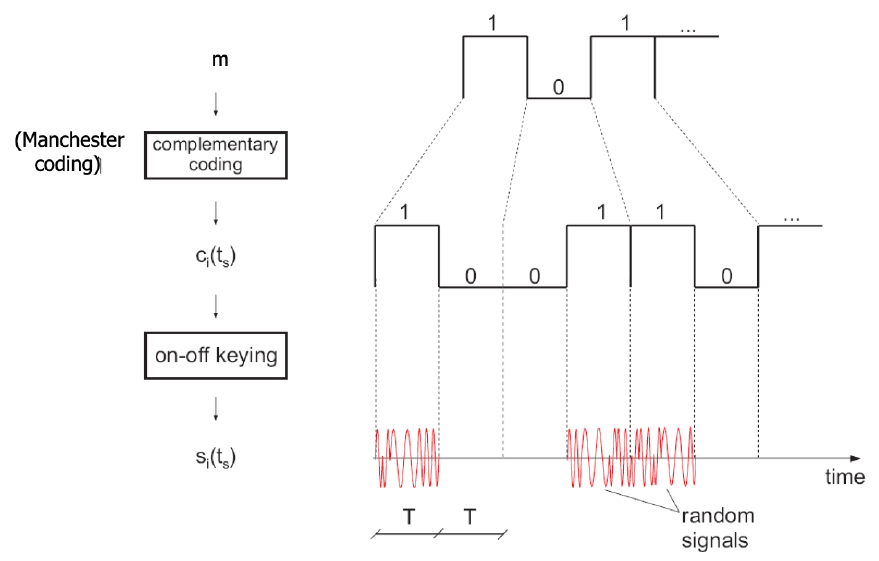
\includegraphics[scale=0.4]{images/7-integrity-code.png}
	\caption{Integrity Codes}
	\label{fig:integrity-code}
\end{figure}

\paragraph{Analysis}
\begin{itemize}
	\item The attacker can easily change $0 \rightarrow 1$ in the raw/keyed signal.
	They can change $1 \rightarrow 0$ only with small probability (assuming signal annihilation is hard).%
	\footnote{thgoebel: Why is this so? Just a couple of slides ahead it was explained that signal annihilation is doable?}
	\item How to handle arbitrary length messages?
	Solution: Use i-delimiters between messages. In Manchester encoding e.g. 111000.
	\item Slow. Solution: broadcast hash of message using integrity codes, use another faster channel for the full message.
\end{itemize}

